\documentclass[12pt]{article}
\usepackage[utf8]{inputenc}
\usepackage[english,russian]{babel}
\usepackage[T2A]{fontenc}
\usepackage{amsmath}
\usepackage{amssymb}
\usepackage{amsfonts}
\usepackage{xcolor}
\usepackage{enumitem}
\usepackage[top=2cm, bottom=2cm, left=2cm, right=2.5cm]{geometry}
\usepackage{lastpage}
\usepackage{fancyhdr}
\usepackage{mathrsfs}
\usepackage{multicol}
\usepackage[hidelinks]{hyperref}
\usepackage{tikz}
\usepackage{wasysym}
\usepackage{amsmath}
\usepackage[most]{tcolorbox}
\usepackage{parskip}
\graphicspath{{images/}}
\usepackage{graphicx}
\usepackage{hyperref}


\usepackage{fontspec}
\setmainfont{Helvetica}
% \setmainfont{CMU Bright}
% \setmainfont{CMU Serif}

\hypersetup{
    colorlinks=true,
    linkcolor=cyan, % blue
    filecolor=magenta,      
    urlcolor=cyan,
    pdftitle={HW1 Dmitry Uspenskiy},
    pdfpagemode=FullScreen,
}

\newcommand{\imgh}[3]
{
\begin{figure}[h]
\center{\includegraphics[width=#1]{#2}}
\caption{#3}
\label{ris:#2}
\end{figure}
}

\newcommand{\condition}[1]
{
\begin{tcolorbox}[enhanced jigsaw,
    sharp corners,
    boxrule=0.5pt, 
    colback=white!30!white,   
    borderline={0.5pt}{-2pt}{black,solid} % 0.5pt linewith, -2pt outside, black solid linestyle
]
#1
\end{tcolorbox}
}

% \setcounter{section}{-1} %Нумерация с 0
\hyphenpenalty=10000

\pagestyle{fancyplain}
\headheight 35pt
\rhead{\textbf{Выполнили:} Успенский Д. А. \\ Беляев И. А. \\ Карбаев С. А. \\ \textbf{Группа:} 208}
\chead{\textbf{\large КТ 1} \\ [3ex] }
\lhead{ФКН ВШЭ \\ Автоматическая Обработка Текста \\ Осенний семестр 2023 \\ } 
\lfoot{}
\cfoot{}
\rfoot{\small\thepage}
\headsep 3em

\begin{document}
\tableofcontents
\newpage

\section{Описание предметной области и постановка задачи}
В качестве проекта мы выбрали \href{https://semantic-textual-relatedness.github.io/}{\textit{Task 1: Semantic Textual Relatedness (STR)}}, где предлагается решить задачу по автоматическому определению степени семантической связи между парами предложений на различных языках.

\subsection{Введение в предметную область}
\textbf{Semantic Textual Relatedness} (семантическая текстовая родственность) показывает степень, в которой две единицы языка, такие как слова, фразы или предложения, близки по своему значению. Это мера того, насколько семантически схожи или родственны две лингвистические единицы друг другу. Задача измерения этой связи возникает естественным образом при работе с текстовыми данными.

Применения меры семантического сходства:
\begin{itemize}
    \item \textbf{Лингвистические}
    \begin{itemize}
        \item изучение отношения между различными языковыми единицами
        \item измерение тесктовой связности
        \item сравнение стиля текстов на различных языках
    \end{itemize}

    \item \textbf{NLP}
    \begin{itemize}
        \item поиск информации в тексте
        \item обобщение документов
        \item оценка методологий: инструмент сравнения с groud truth текстами
        \item создание датасетов: наборы данных семантической текстовой связанности, таких как STR-2022 (Mohamed Abdalla et. al. , 2023)
    \end{itemize}
\end{itemize}

\subsection{Постановка задачи}
На соревновании мы выбрали трек \textit{A: Supervised}. Необходимо обучить модель, которая предсказываеи STR двух предложений. Доступны тренировчный и тестовый датасеты на английском.

\newpage

\section{Описание датасета}
\subsection{Структура датасета}
Каждый объект в датасете представляет собой пару предложений и оценку, отражающую степень семантической текстовой связи между двумя предложениями. Баллы могут варьироваться от 0 (максимально не связаны) до 1 (максимально связаны). Эти оценки были определены путем ручного аннотирования. В частности, использовался метод \textit{comparative annotation}, чтобы избежать известных ограничений традиционных методов оценки сходства.

**пример аннотации** 

\subsection{Измерение качества}
Официальной метрикой оценки для этого задания является коэффициент ранговой корреляции Спирмена, который отражает, насколько хорошо предсказанные системой рейтинги тестовых экземпляров согласуются с суждениями человека.

\newpage

\section{Предварительный анализ данных}
\subsection{График распределения}
Посмотрим на график распределения целевой переменной

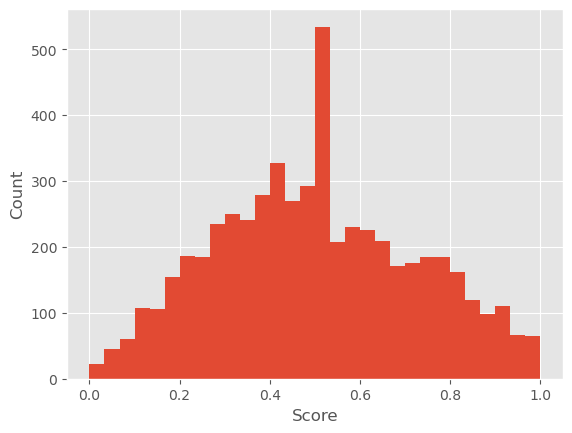
\includegraphics[width=0.7\linewidth]{распределение}

Получили что-то немного похожее на нормальное распределение

\subsection{Базовое решение}

Сначала попробуем что-то простое. Составим словарь слов каждого из 2 предложений и посмотрим сколько слов в них пересекаются. Затем, для получения целевой переменной, поделим найденное число на общее количество слов в каждом предложении.

Удалим из наших предложений самые распространенные слова (если 'the' есть в каждом предложении, более похожими они не станут) и ненужные символы.

В итоге мы получили результат    




\newpage

\section{Обзор литературы}

 \begin{enumerate}
	\item  \href{https://www.researchgate.net/publication/272088094_A_SEMANTIC_SIMILARITY_MEASURE_BETWEEN_SENTENCES}{A SEMANTIC SIMILARITY MEASURE BETWEEN SENTENCES}
	
	
	\item обобщение документов
	\item оценка методологий: инструмент сравнения с groud
\end{enumerate}



\newpage

\section{Описание выбранной архитектуры}
\newpage


\section{Описание полученных результатов}
\newpage


\section{Направления дальнейшей работы}
\newpage


\section{Источники}
\begin{itemize}
    \item Nedjma Ousidhoum et. al. SemEval 2024 Task 1: Semantic Textual Relatedness (STR)
   \href{https://semantic-textual-relatedness.github.io/}{Source}

   \item Mohamed Abdalla et. al. , 2023 "What Makes Sentences Semantically Related?
   A Textual Relatedness Dataset and Empirical Study"
\end{itemize}
\end{document}
